%%%%%%%%%%%%%%%%%%%%%%%%%%%%
% CHAPTER 7 - DISCUSSION of THEORY: ONGOING
%%%%%%%%%%%%%%%%%%%%%%%%%%%%
%%%%%%%%%%%%%%%%%%%%%%%%%%%%%%%%%%%%%%%%%%%%%%%%%%%%%%%%%%%%%%%%%%%%%%%%%%%%%%%%%%%%%%%%%%
% Richard Boardman PhD Thesis: Improving Tool Support for Personal Information Management
%%%%%%%%%%%%%%%%%%%%%%%%%%%%%%%%%%%%%%%%%%%%%%%%%%%%%%%%%%%%%%%%%%%%%%%%%%%%%%%%%%%%%%%%%%

% \newpage
%%%%%%%%%%%%%%
% ONGOING
%%%%%%%%%%%%%%
%%%%%%%%%%%%%%%%%%%%%%%%%%%%%%%%%%%%%%%
\subsection{PIM as an Ongoing Activity}
\label{discussion:ongoing}
%%%%%%%%%%%%%%%%%%%%%%%%%%%%%%%%%%%%%%%
% The previous two sections have discussed PIM as a \textit{cross-tool} and \textit{supporting} activity in turn.
This section views PIM from a third theoretical perspective, as an \textit{ongoing} activity.
%%%%%%%%%%%%%%%%%%%%%%%%%%%%%%%%%%%%%%%%%%%%%
% PIM as continuous, background activity
%%%%%%%%%%%%%%%%%%%%%%%%%%%%%%%%%%%%%%%%%%%%%
The main study reported in \textbf{Chapter~\ref{chapter:main-study}} tracked PIM behaviour over time in terms of four PIM sub-activities: acquisition, organization, maintenance and retrieval. \textbf{Figure~\ref{fig:discussion:ongoing-model-SIMPLE}} illustrates how each of these sub-activities can be viewed on a both a short-term and long-term time-scale:

%%%%%%%%%%%%%%%%%%%%%%%%%%%%%%%%%%%%%%%%%%%%%%%%%%%%%%%%
% Break-down into parallel threads and one-off events
%%%%%%%%%%%%%%%%%%%%%%%%%%%%%%%%%%%%%%%%%%%%%%%%%%%%%%%%
% PIM is in turn made up of parallel threads corresponding to the PIM sub-activities: .
% Therefore can analyse in terms of a sequence of short-term discrete events corresponding to the acquisition, organization, maintenance and retrieval of specific items. Consider PIM as one-off local events, e.g. retrieving an item from an email collection.
% The sub-activities that make up PIM, , can all be considered to be ongoing activities, as shown in .
%%%%%%%%%%%%%%%%%%%%%%%%%%%%%%%%%%%%%%%%%%%%%%%%%%
% Model of at two levels: short-term, long-term
%%%%%%%%%%%%%%%%%%%%%%%%%%%%%%%%%%%%%%%%%%%%%%%%%%
% PIM can be considered from two perspectives, an ongoing long-term one, and from a short-term time-scale of discrete events: 
\begin{enumerate}

% PIM can also be considered to be made up of a sequence of one-off events that happen at a specific point in time.  
\item From a \textit{short-term} perspective, each sub-activity consists of a sequence of discrete events. For example, the acquisition sub-activity within a file context consists of a series of file-saving events. 
% The relative frequency of PIM sub-activities is considered. 
\textbf{Section~\ref{disc:study-discussion:growth}} noted the relative frequency of a user performing the four sub-activities. This is reflected in \textbf{Figure~\ref{fig:discussion:ongoing-model-SIMPLE}}: whilst acquisition and retrieval occur frequently, organization and maintenance are more sporadic.

\item Alternatively, from a long-term perspective, PIM can be viewed as four continuous threads of behaviour, each corresponding to the four PIM sub-activities and consisting of a sequence of discrete events.  PIM behaviour over time is therefore the combination of the four interleaved sub-activities, amounting to a continuous, background thread of activity.   In the extreme, PIM behaviour is now \textit{lifelong} since users can collect and store information over their entire lifetime~\citep{bell:02,dix:02}.  
% Each thread can be decomposed into a sequence of discrete events.

\end{enumerate}


%%%%%%%%%%%%%%%%%%%%%%%%%%%%%%%%%%%%%%
% %%%%%%%%%%%%%%%%%%%%%%%%%%%%%%%%%%%%
% FIGURE - An ongoing model of PIM
% %%%%%%%%%%%%%%%%%%%%%%%%%%%%%%%%%%%%
%%%%%%%%%%%%%%%%%%%%%%%%%%%%%%%%%%%%%%
\begin{figure}[hbtp]
	\begin{center}
		\leavevmode
		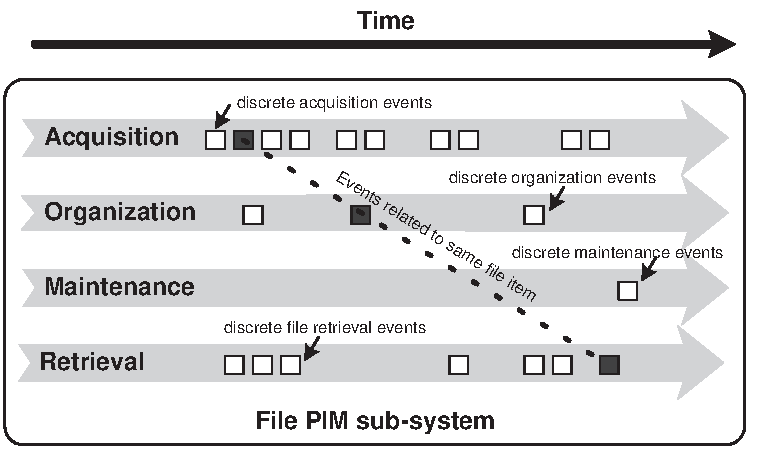
\includegraphics[height=6cm]{pictures/discussion/PIM-ongoing-model-SIMPLE.pdf}
	\end{center}
	\caption{PIM as an ongoing activity, consisting of four parallel threads corresponding to the four PIM sub-activities}
	\label{fig:discussion:ongoing-model-SIMPLE}
\end{figure}

%%%%%%%%%%%%%%%%%%%%%%%%%%%%%%
% PIM BEHAVIOUS AS A WHOLE
%%%%%%%%%%%%%%%%%%%%%%%%%%%%%%
Following from the long-term view of PIM, a number of discussion points can be raised.  
\begin{itemize}

%%%%%%%%%%%%%%%%%%%%
% STRATEGIES
%%%%%%%%%%%%%%%%%%%%
% PIM can be considered as a continuous, background thread of activity, carried out in support of a user's production tasks. Note that PIM can be considered to be distributed both over tools and over time.
\item Just as production activities may evolve over time (consider the stages of writing a report), so may the activities supporting them.  For example, \textbf{Section~\ref{main-study:results:changes}} described how PIM strategies may change over time.  The very notion of a PIM strategy suggests that behaviour is pre-planned and consistent.  However, the supporting nature of PIM means that users rarely devote time to planning and executing changes in strategy.  Instead, PIM strategies are not pre-determined, but the amalgam of many spur-of-the-moment discrete events.  For example, Participant 2 in the exploratory study reported: \textit{``I start working with something, create a new dedicated area, and then forget about it''}.  In the past, when researchers have talked about ``organizing strategies'', they are typically describing \textit{average behaviour over the long-term}
\footnote{The term \textit{average} acknowledges the multiple strategies employed by many users to manage different types of information, e.g. filing information related to some production activities but not others (see \textbf{Section~\ref{exp-study:discussion:multiple-strategies}}).}.
% As discussed in \textbf{Chapter~\ref{chapter:exploratory_study}}, users may employ different strategies }.  %  Furthermore, such low-level strategies may change over time.  
% In addition, the word ``strategy'' has the connotation that users devote time to selecting that strategy. 




% .  Whilst PIM is an ongoing thread of activity which evolves over time, information retrieval 
\item The long-term perspective allows PIM to be contrasted with information retrieval, which is typically considered to be a one-off discrete event.  In contrast, Wilson's ``human information behaviour''~\citep{wilson:00} is equivalent to the ongoing retrieval sub-activity thread, portrayed here as one aspect of PIM.  

%%%%%%%%%%%%%%%%%%%%%%%%%%%%%%%%%%%%%%%%%%%%%
% Inter-relating the sub-activities of PIM}: 
%%%%%%%%%%%%%%%%%%%%%%%%%%%%%%%%%%%%%%%%%%%%%
% \item Inter-equivalence of storage and retrieval (on-demand organization) DISCUSS: THINK: retrieval is effectively organization (enforcing a particular view of the data-set) at "query time". On-demand organization.
%%%%%%%%%%%%%%%%%%%%%%%%%%%%%%%%%%%%%%%%%%%%%%%%%%%%%%%%%%%%%%%%%%%%%%%%%%%%%%%%%%
%%%%%%%%%%%%%%%%%%%%%%%%%%%%%%%%%%%%%%
% Linking events across the threads
%%%%%%%%%%%%%%%%%%%%%%%%%%%%%%%%%%%%%%
% The long-term perspective is important as .  The acquisition of an item, may correspond to a retrieval event months later: at two different points in time.
% PIM is more continuous than information-seeking although made up of discrete events over time.  By considering PIM over time, it can be seen that events in separate threads, that occur at different times are related.  
% an example acquisition event is saving a newly-created file, which may be retrieved at a later date via a distinct retrieval event.  An example of this is indicated by the black squares in 
% Within a specific PIM sub-system, the individual acquisition events in a particular sub-activity amount to the user's total acquisition over time. 
\item The four threads in \textbf{Figure~\ref{fig:discussion:ongoing-model-SIMPLE}} are not independent -- they each represent a series of actions performed within a single collection of information.  Indeed, discrete events in two different threads may be associated by involving the same item of information.  To illustrate this point, the black squares in \textbf{Figure~\ref{fig:discussion:ongoing-model-SIMPLE}} indicate the association between the acquisition, storage and later retrieval of a particular item.  

The nature of one sub-activity can influence how users perform other sub-activities. For example, the rate at which users acquire items, influences their choice of organization, maintenance and retrieval strategies.
% In turn, if users organize items within folders, this leads to the need to organize those folders as well as the items they contain.
Also, organization and maintenance have a strong influence on retrieval.  Several participants commented that maintaining their collections (e.g. tidying, deleting items) could make it harder to find items.  % It is noted that Barreau's division of PIM into four distinct sub-activities may obscure such inter-relationships. %
% \begin{itemize}
%%%%%%%%%%%%%%%%%%%%%%%%%%%%%%%%%%%%%%%%%%%%%%%
% The sub-activities influence one another
% \item Several users mentioned downside of org for search/sort (I try to minimise structure as I find by sorting on date and sender metadata to get a flexible view)
% \item Cost-benefit trade-off in storage/retrieval. When to invest time. Many users perceive that org leads to faster retrieval.  But also that no org is better.
%%%%%%%%%%%%%%%%%%%%%%%%%%%%%%%%%%%%%%%%%%%%%%%
% * Acquisition - leads to clutter and need to organize. Over time, shift from item-clutter to folder-clutter
%%%%%%%%%%%%%%%%%%%%%%%%%%%%%%%%%%%%%%%%%%%%%%%%%%%%%%%%%%%%%%%%%	
% The sub-activities overlap
% Acquisition (allocation of value) as ``not deleting'' (email)
% Acquisition as implicit storage/organization (implicit metadata). Explicit organization as extra
%%%%%%%%%%%%%%%%%%%%%%%%%%%%%%%%%%%%%%%%%%%%%%%%%%%%%%%%%%%%%%%%%
% \item The sub-activities often overlap. For example, in email deciding what new messages to delete from the inbox (inbox maintenance), can be viewed as a form of acquisition (deciding what to add to the collection).
%%%%%%%%%%%%%%%%%%%%%%%%%%%%%%%%%%%%%%%%%%%
% Need better definition of acquisition
%%%%%%%%%%%%%%%%%%%%%%%%%%%%%%%%%%%%%%%%%%%
% \item Compare acquisition of new item, and re-saving edited version of one that already exists
% * Acquisition - too easy to acquire
% \end{itemize}

\end{itemize}




%%%%%%%%%%%%%%%%%%%%%%%%%%%%%%%%%%%%%%%%%%%%%%%%%%%%%%%%%%%%%%%%%%%%%%%%%%%%%%%%%
% THINK: relationship with information retrieval here rather than in Chapter 2}
%%%%%%%%%%%%%%%%%%%%%%%%%%%%%%%%%%%%%%%%%%%%%%%%%%%%%%%%%%%%%%%%%%%%%%%%%%%%%%%%%%


%%%%%%%%%%%%%%%%%%%%%%%%%%%%%%%%%%%%%%%%%%%%%%%%%%%%%%%
\subsubsection{Extending the Theoretical Framework}
%%%%%%%%%%%%%%%%%%%%%%%%%%%%%%%%%%%%%%%%%%%%%%%%%%%%%%%

\textbf{Figure~\ref{fig:discussion:ongoing-model}} shows the theoretical framework extended to accommodate all three perspectives discussed in this section: (1) \textit{cross-tool}, (2) \textit{supporting}, and (3) \textit{ongoing}.  % It can be argued that previous work in this area has not focused on these aspects, so each highlights promising routes for future work in terms of theoretical development or empirical investigation. 


% Now the theoretical framework shown in \textbf{Figure~\ref{fig:design:PIM-production-simple}} is extended to reflect the ongoing perspective on PIM outlined above.
% LINK TO CROSS-TOOL DISCUSSION: added need for cross-tool coordination as PIM is distributed over time AND across too
% The combined framework is shown in \textbf{Figure~\ref{fig:discussion:ongoing-model}}. 
The figure shows two example production activities (A and B) and the associated PIM activity.  The squares and triangles refer to PIM events relating to production activity A and B, respectively.   PIM is also shown to be distributed \textit{across tools}, and \textit{over time} (horizontal axis).    The figure reflects variations in the frequency of PIM events between tools.  Due to the discretionary nature of PIM, events in the parallel threads, relating to various production activities, may be interleaved arbitrarily.

%%%%%%%%%%%%%%%%%%%%%%%%%%%%%%%%%%%%%%
% %%%%%%%%%%%%%%%%%%%%%%%%%%%%%%%%%%%%
% FIGURE - An ongoing model of PIM
% %%%%%%%%%%%%%%%%%%%%%%%%%%%%%%%%%%%%
%%%%%%%%%%%%%%%%%%%%%%%%%%%%%%%%%%%%%%
\begin{figure}[hbtp]
	\begin{center}
		\leavevmode
		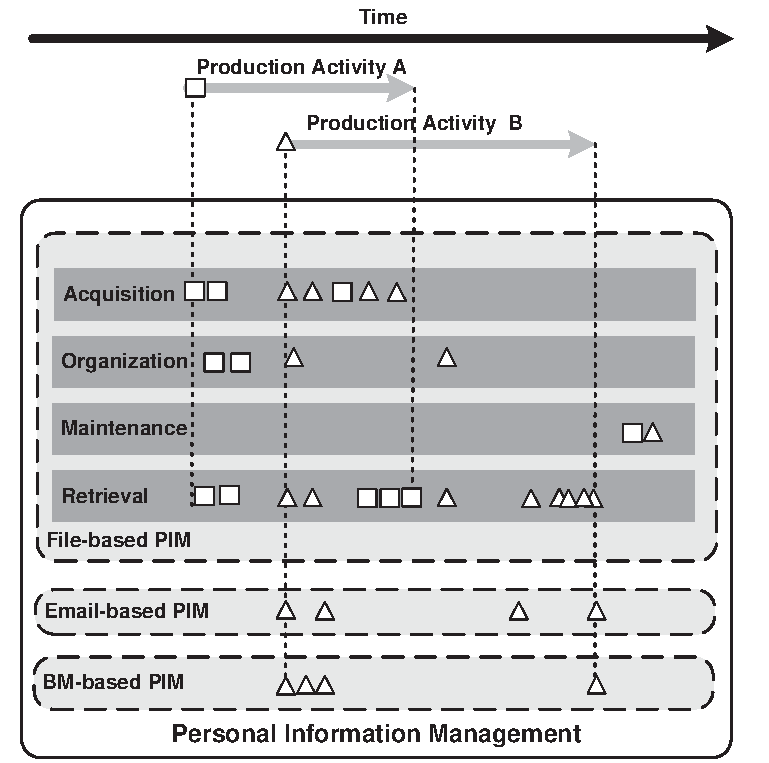
\includegraphics[height=10cm]{pictures/discussion/PIM-ongoing-model.pdf}
	\end{center}
	\caption{Theoretical framework extended to reflect the cross-tool, supporting, and ongoing nature of PIM}
	\label{fig:discussion:ongoing-model}
\end{figure}

%%%%%%%%%%%%%%%%%%%%%%%%%%
% LINK TO OTHER SECTIONS
%%%%%%%%%%%%%%%%%%%%%%%%%%
%The next section considers how PIM behaviour may evolve over time.  Such insights may shed light on the uptake of new tools by users.
% Methodological implications for evaluating PIM-tools are considered in \textbf{Section~\ref{discussion:methodological-discussion}}.


%%%%%%%%%%%%%%%%%%%%%%%%%%%%%%%%%%%%%%%%%%%%%%%%%%%%%%%%%%%%%%%%%%%%%%%%%%%%%%%%%%%%%%%%%%%%%%%%%%%%%%%%%%%%%%%%%
%%%%%%%%%%%%%%%%%%%%%%%%%%%%%%%%%%%%%%%%%%%%%%%%%%%%%%%%%%%%%%%%%%%%%%%%%%%%%%%%%%%%%%%%%%%%%%%%%%%%%%%%%%%%%%%%%
%%%%%%%%%%%%%%%%%%%%%%%%%%%%%%%%%%%%%%%%%%%%%%%%%%%%%%%%%%%%%%%%%%%%%%%%%%%%%%%%%%%%%%%%%%%%%%%%%%%%%%%%%%%%%%%%%
%%%%%%%%%%%%%%%%%%%%%%%%%%%%%%%%%%%%%%%%%%%%%%%%%%%%%%%%%%%%%%%%%%%%%%%%%%%%%%%%%%%%%%%%%%%%%%%%%%%%%%%%%%%%%%%%%


%%%%%%%%%%%%%%%%%%%%%%%%%
\subsection{Towards a Theory of PIM}
\label{discussion:towards-theory}
%%%%%%%%%%%%%%%%%%%%%%%%%

%%%%%%%%%%%%%%%%%%%%%%%%%%%%%%%
% Talking about INFORMATION
%%%%%%%%%%%%%%%%%%%%%%%%%%%%%%%
The framework in \textbf{Figure~\ref{fig:discussion:ongoing-model}} illustrates three important aspects of PIM that have emerged over the course of this research programme.  Note that the framework is not intended to represent a complete model of PIM.  Instead, it is presented to illustrate three areas that must be accommodated in future theoretical work in this area.  The framework also highlights the analytical complexity of PIM as a HCI phenomenon.  One way to deal with such complexity, may be to develop an inter-linked set of theories, rather than a monolithic one~\citep{barnard:00}.

There are also many other areas in which the theoretical basis of PIM could be improved.  One other area suggested by \citet{Whittaker-rta:00} is to improve the \textit{descriptive vocabulary} for talking about personal information.  The author echoes this call.  This research points at one fundamental area in need of attention -- that is the need for a richer vocabulary to describe items of personal information beyond \textit{technological format}, and \textit{lifetime of use}~\citep{bn:95}. For example, \textbf{Chapter~\ref{chapter:exploratory_study}} advocated that the term ``archived'' is misleading, since most users do not archive explicitly.  Two alternative sets of terms are suggested:
\begin{enumerate}
	\item \textit{Information usefulness} -- \textit{active} (relating to current production activities, including ephemeral and working items), \textit{dormant} (inactive, potentially useful), \textit{not useful} (should be deleted), and \textit{un-assessed} (e.g. new emails).
	\item \textit{Information ownership} -- \textit{mine} (including self-created files, and items that have been assessed as having value, e.g. filed email), and \textit{``not-mine''} (e.g. much of the email inbox, and information on the internet).
\end{enumerate}

The subsequent sections of this discussion chapter draw on the theoretical framework developed over \textbf{Sections~\ref{discussion:cross-tool}} to \textbf{\ref{discussion:ongoing}}. Firstly, \textbf{Section~\ref{discussion:design-guidelines-discussion}} revisits the WM evaluation in lieu of the discussion of PIM as a supporting activity.  A number of design implications are discussed, focusing on improving integration between PIM-tools.  % Then, \textbf{Section~\ref{discussion:methodological-discussion}} considers methodological implications that can be drawn from the three aspects of PIM discussed above.

%%%%%%%%%%%%%%%%%%%%%%%%%%%%%%%%%%%%%%%%%%%%%%%%%%%%%%%%%%%%%%%%%%%%%%%%%%%%%%%%%%%%%%%%%%%%%%%%%%%%%%%%%%%%%%%%%
%%%%%%%%%%%%%%%%%%%%%%%%%%%%%%%%%%%%%%%%%%%%%%%%%%%%%%%%%%%%%%%%%%%%%%%%%%%%%%%%%%%%%%%%%%%%%%%%%%%%%%%%%%%%%%%%%
%%%%%%%%%%%%%%%%%%%%%%%%%%%%%%%%%%%%%%%%%%%%%%%%%%%%%%%%%%%%%%%%%%%%%%%%%%%%%%%%%%%%%%%%%%%%%%%%%%%%%%%%%%%%%%%%%
%%%%%%%%%%%%%%%%%%%%%%%%%%%%%%%%%%%%%%%%%%%%%%%%%%%%%%%%%%%%%%%%%%%%%%%%%%%%%%%%%%%%%%%%%%%%%%%%%%%%%%%%%%%%%%%%%

%%%%%%%%%%%%%%%%%%%%%%%%%%%%%
% END: THEORETICAL FRAMEWORK
%%%%%%%%%%%%%%%%%%%%%%%%%%%%%




